\documentclass[a4paper,11pt]{article}
\usepackage[T1]{fontenc}
\usepackage[utf8]{inputenc}
\usepackage{lmodern}
\usepackage[francais]{babel}
\usepackage{graphicx}
\usepackage{listings}

% pour definir des couleurs
\usepackage{xcolor}

%couleur
\usepackage{color}
\usepackage{multicol}

% code color
\definecolor{ligthyellow}{RGB}{250,247,220}
\definecolor{darkblue}{RGB}{5,10,85}
\definecolor{ligthblue}{RGB}{1,147,128}
\definecolor{darkgreen}{RGB}{8,120,51}
\definecolor{darkred}{RGB}{160,0,0}

\lstset{
    language=Python,
    captionpos=b,
    extendedchars=true,
    frame=lines,
    numbers=left,
    numberstyle=\tiny,
    numbersep=5pt,
    keepspaces=true,
    breaklines=true,
    showspaces=false,
    showstringspaces=false,
    breakatwhitespace=false,
    stepnumber=1,
    showtabs=false,
    tabsize=3,
    basicstyle=\small\ttfamily,
    backgroundcolor=\color{ligthyellow},
    keywordstyle=\color{ligthblue},
    morekeywords={include, printf, uchar},
    identifierstyle=\color{darkblue},
    commentstyle=\color{darkgreen},
    stringstyle=\color{darkred},
}

\title{Approche de la logique floue}
\author{Elliot Vanegue}

\begin{document}

\maketitle

\section{Introduction}
Lors de ce TP, nous allons nous familiariser avec les concepts principaux de la logique floue.
La logique floue repose sur un système de propositions dont la valeur est dans l'intervalle [0,1] contrairement aux logiques modales qui reposent sur un système binaire. 

\section{Fonction d'appartenance}
Dans un premier temps, nous programmons trois ensembles flous représentant des intervalles de température.
Pour cela nous définissons une fonction par intervalle afin de définir sa courbe. Dans ces fonctions, nous 
distinguons trois cas possibles :
\begin{itemize}
  \item Un intervalle où l'ensemble est vrai (ordonnée = 1)
  \item Un intervalle où l'ensemble est faux (ordonnée = 0)
  \item Un intervalle où l'ensemble a un degré d'incertitude entre 0 et 1
\end{itemize}
Nous obtenons ainsi le graphique de la Fig. \ref{fig:GraphiqueFlou} 

\begin{figure}[!h]
  \begin{center}
    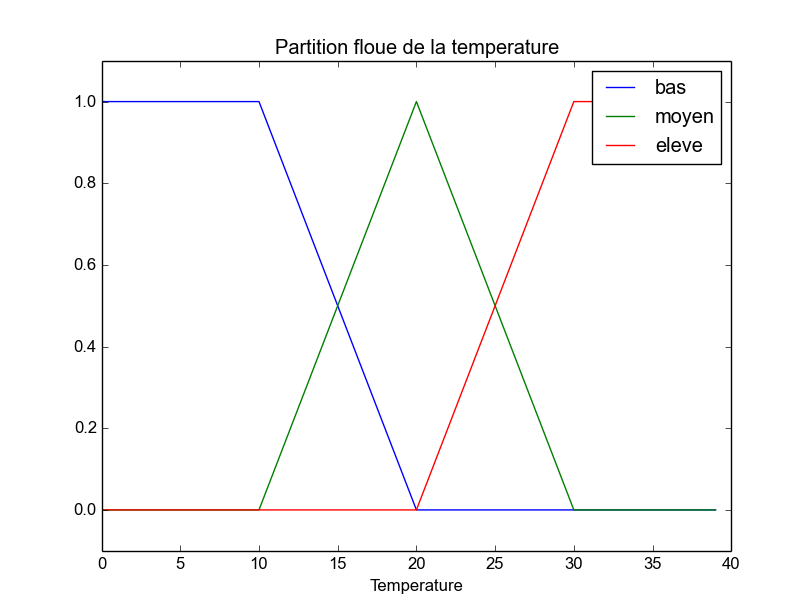
\includegraphics[width=9cm]{tempFlou.png}
    \caption{Graphique de la partition floue de l'exemple \og Température \fg}
    \label{fig:GraphiqueFlou}
  \end{center}
\end{figure}

\begin{lstlisting}[caption=Fonction de l'ensemble température basse]
  def CalcTempB(i):
    if(i < 10):
        return 1.0
    elif(i<20):
        return 1.0 - ((1.0/10.0) * (i-10.0))
    else:
        return 0.0
\end{lstlisting}

Cela nous permet ainsi de déterminer les degrés d'appartenance de la température $16\deg$ pour chaque sous 
ensemble (voir Tab. \ref{tab:temp16}).
\begin{table}[!h]
  \label{tab:temp16}
  \begin{center}
    \begin{tabular}{|c|c|c|}
      \hline
       classe & degré d'appartenance\\
       \hline
       basse & 0.4\\
       moyenne & 0.6\\
       élevé & 0.0\\
    \end{tabular}
    \caption{Résultat du degré d'appartenance de la température 16 dans chaque ensemble}
  \end{center}
\end{table}

\section{Opérateurs de la logique floue}
Il est possible de définir des opérateurs permettant de récupérer en sortie les valeurs maximum ou 
minimum de deux ensembles. Pour cela nous créons les fonctions suivantes :
\begin{lstlisting}[caption=Opérateur min]
 def Opmin(tab1, tab2):
  size = range(0, min(len(tab1), len(tab2)))
  result = []
  for i in size:
      step = [tab1[i], tab2[i]]
      result.append(min(step))
  return result
\end{lstlisting}

\begin{lstlisting}[caption=Opérateur max]
 def Opmax(tab1, tab2):
  size = range(0, min(len(tab1), len(tab2)))
  result = []
  for i in size:
      step = [tab1[i], tab2[i]]
      result.append(max(step))
  return result
\end{lstlisting}

\begin{figure}[!h]
  \begin{center}
    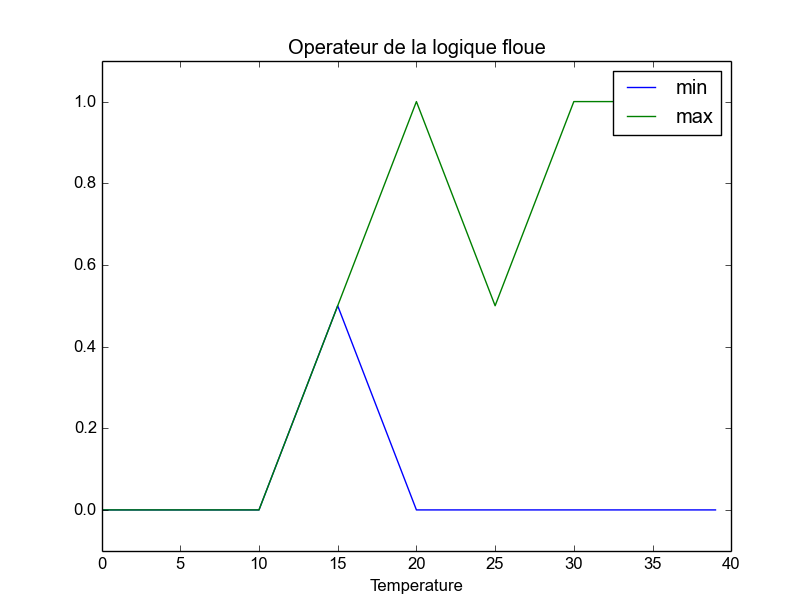
\includegraphics[width=9cm]{operateurFlou.png}
    \caption{Graphique des fonctions min et max de la logique floue}
    \label{fig:operateur}
  \end{center}
\end{figure}

Dans la Fig. \ref{fig:operateur}, la courbe bleue représente la fonction min entre les sous-ensembles
température moyenne et température élevée, et la courbe verte représente la fonction max pour les mêmes
sous-ensembles que la courbe bleue.

\section{Implication floue}
A partir de la règle \og si température basse alors chauffer fort \fg , nous utilisons l'implication
de Mamdani pour construire la sortie \og puissance de chauffe \fg . L'implication de Mamdani dit que l'ensemble
flou de sortie correspond au minimum entre une fonction et la valeur recherchée. En appliquant
ce principe nous obtenons le sous-ensemble de la Fig. \ref{fig:mamdani} où la valeur maximum est 0.8, car 0.8 est la valeur 
d'incertitude de la température 12\degre.

\begin{figure}[!h]
  \begin{center}
    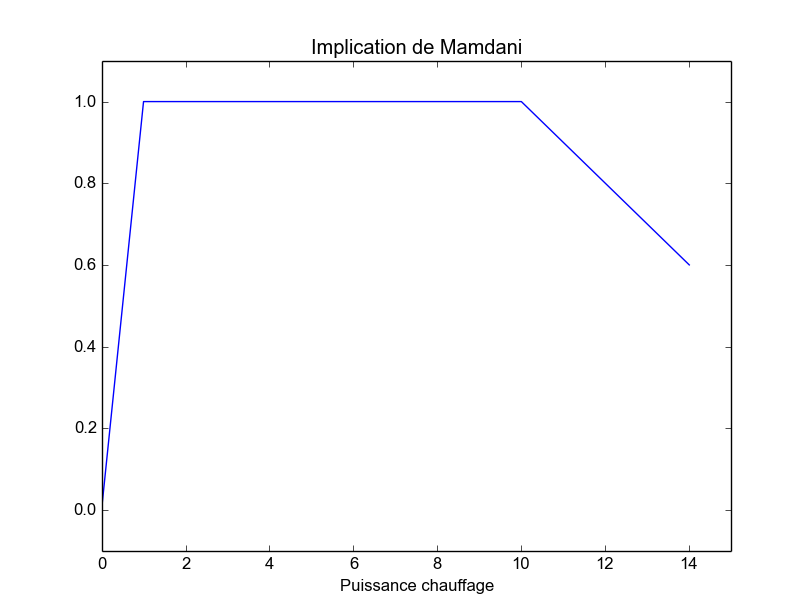
\includegraphics[width=9cm]{mamdani.png}
    \caption{Sortie \og puissance de chauffe fuzzifiée \fg}
    \label{fig:mamdani}
  \end{center}
\end{figure}
\newpage
\section{Conclusion}
Comme nous avons pu le voir, la logique floue est assez simple à implémenter et permet de modéliser des situations
complexes dans des fonctions. 
\end{document}
